\section{Step 3: Live Gateway}\label{sec:live}

\emph{What an offline score hides.} A gateway classifies flows exported while packets still arrive, not flows from a finished file. Equal scores do not show that both see the same flows, so we check fidelity flow by flow.

\subsection{Testbed}\label{sec:testbed}

The testbed runs Mininet~2.3.0~\cite{lantz2010mininet} with Open vSwitch (OVS)~\cite{pfaff2015ovs} under WSL2 Ubuntu~24.04 on a laptop (i5-8350U, no GPU). In the topology h1--s1--gw--s2--h2, h1 replays traffic with tcpreplay at $\times1.0$ timing, and the gateway gw captures on its s1-facing interface. The gateway runs NFStream~6.6.0 in live mode with the offline settings, a single meter and a 64\,MB capture buffer. Exported flows are classified in micro-batches (256 flows or 50\,ms) by the deployed tree; each flow receives one \emph{verdict}, its predicted class. The gateway can install OVS drop rules for both directions of a host pair (Section~\ref{sec:response}).

\emph{Windows and harness.} For each capture we cut one 60\,s window that starts 1\,s after the last training flow started, so all replayed traffic comes from the test period. Boundary-spanning connections are removed on both the offline and the live side; the offline reference is NFStream run on the same window file. After each window the harness waits until the gateway is idle and clears OVS blocks, per-pair verdict counts and ARP state, since the sessions reuse addresses. The first no-limit run (run~1) and the one-core run used an earlier harness without the quiet wait and the reset. A cgroup quota (\texttt{systemd-run}) sets the gateway's CPU budget: no limit, one core or half a core.

\emph{Achieved replay rates.} tcpreplay could not reach the original rate of the heaviest windows: DDoS-SYN (17,424 packets per second, pps) and Mirai (4,782\,pps) were replayed at 52--77\% of it.

\subsection{Fidelity Check}\label{sec:fidelity}

\emph{Flow-by-flow match.} We match live to offline flows by 5-tuple and order of appearance within the 5-tuple, on every run. In run~1 (no CPU limit, ten windows), 148,756 of 148,779 offline flows match one of the 148,884 live flows; per window, 96.62--100\% of the matched flows have identical packet and byte counts, and 97.63--100\% receive the same verdict. Over all seven runs without enforcement, at least 99.98\% of the offline flows match and at least 99.97\% of the matched flows receive the same verdict. Macro-F1 over run~1's windows (not comparable to the test-set score) is 0.804 both offline and live.

\emph{Packet accounting.} The packet ratio (packets in live over offline flows, per window) lies between 0.9919 and 1.0064, and NFStream reported zero kernel drops, including in the DDoS-SYN and Mirai windows.

\emph{Delay.} Inference takes 0.44\,ms per batch (medians; 209 flows per batch). Delay comes from flow export, as expected for flow-based detection~\cite{hofstede2013realtime}: the median verdict arrives about 15\,s (the idle timeout) after a flow's last packet, and the first verdict for an attacker pair 15--35\,s after its first packet.

\begin{table}[t]
\centering
\caption{Live runs, DDoS-SYN window (offline: 142,724 flows). Replay: achieved rate and its share of the original 17,424\,pps. Same pkts: share of matched flows with identical packet counts. Delay: median verdict after flow end. Macro-F1: live, over the three windows tested at every CPU budget (offline 0.914).}
\label{tab:repeats}
\footnotesize
\setlength{\tabcolsep}{2.5pt}
\begin{tabular}{lrrrccc}
\hline
 & \multicolumn{2}{c}{Replay} & Live & Same & Delay & Macro- \\
Run & pps & \% & flows & pkts & (s) & F1 \\
\hline
No limit 1  & 12,271 & 70.4 & 142,752 & 1.000 & 17.8 & 0.9171 \\
No limit 2  & 11,611 & 66.6 & 160,242 & 0.877 & 30.9 & 0.9155 \\
No limit 3  & 10,936 & 62.8 & 184,483 & 0.708 & 34.0 & 0.9175 \\
One core    & 13,434 & 77.1 & 142,725 & 1.000 & 21.5 & 0.9284 \\
Half core 1 & 12,088 & 69.4 & 142,730 & 1.000 & 75.9 & 0.9175 \\
Half core 2 & 11,831 & 67.9 & 160,475 & 0.876 & 97.0 & 0.9172 \\
Half core 3 & 12,401 & 71.2 & 142,729 & 1.000 & 60.3 & 0.9173 \\
\hline
\end{tabular}
\end{table}

\emph{Repeats: macro-F1 hides flow splitting.} We ran the no-limit and half-core settings three times each and the one-core setting once (Table~\ref{tab:repeats}). Every run captured every packet (zero kernel drops, DDoS-SYN packet ratio 1.00), but flow construction followed the replay rate. At 69\% or more of the original DDoS-SYN rate the live flow count matched offline within 0.02\%; at 63--68\% it was 12--29\% higher, and the share of matched flows with identical packet counts fell to 0.71--0.88, because slower replay stretches inter-packet gaps past the idle timeout and splits connections. Macro-F1 did not move: 0.9155--0.9175 on the three common windows in every run but the one-core one (0.9284), and 0.8038--0.8043 over all ten windows of the no-limit runs. This is Check~3 applied to our own runs: the score hides the loss of flow fidelity, and only the flow-by-flow match shows it. The one-core run's higher score comes from one extra, correctly classified Mirai flow at a lower replay rate.

\emph{CPU budget.} The budget affected verdict delay only in the DDoS-SYN window (Fig.~\ref{fig:delay}), but its load spilled over: with one core, a backlog kept the CPU at about 100\% for 45--60\,s after the flood, into the BruteForce window (mean CPU 40.6\% there, against 0.8\% without a limit), whose median delay still stayed at 15.7\,s. With half a core the gateway needed another 110--163\,s after the gap to clear its backlog, still without drops: CPU pressure caused lag, not loss, but the flood never filled the 64\,MB buffer. These comparisons are confounded: tcpreplay shares the laptop CPU with the gateway, so the replay rate depends on the gateway's load; the one-core run used the earlier harness; and half a core was tested on three windows only. We report them as observations from these runs. Peak memory was 980--1,025\,MB, from NFStream and Python, not from the 222\,KiB tree.

\begin{figure}[t]
\centering
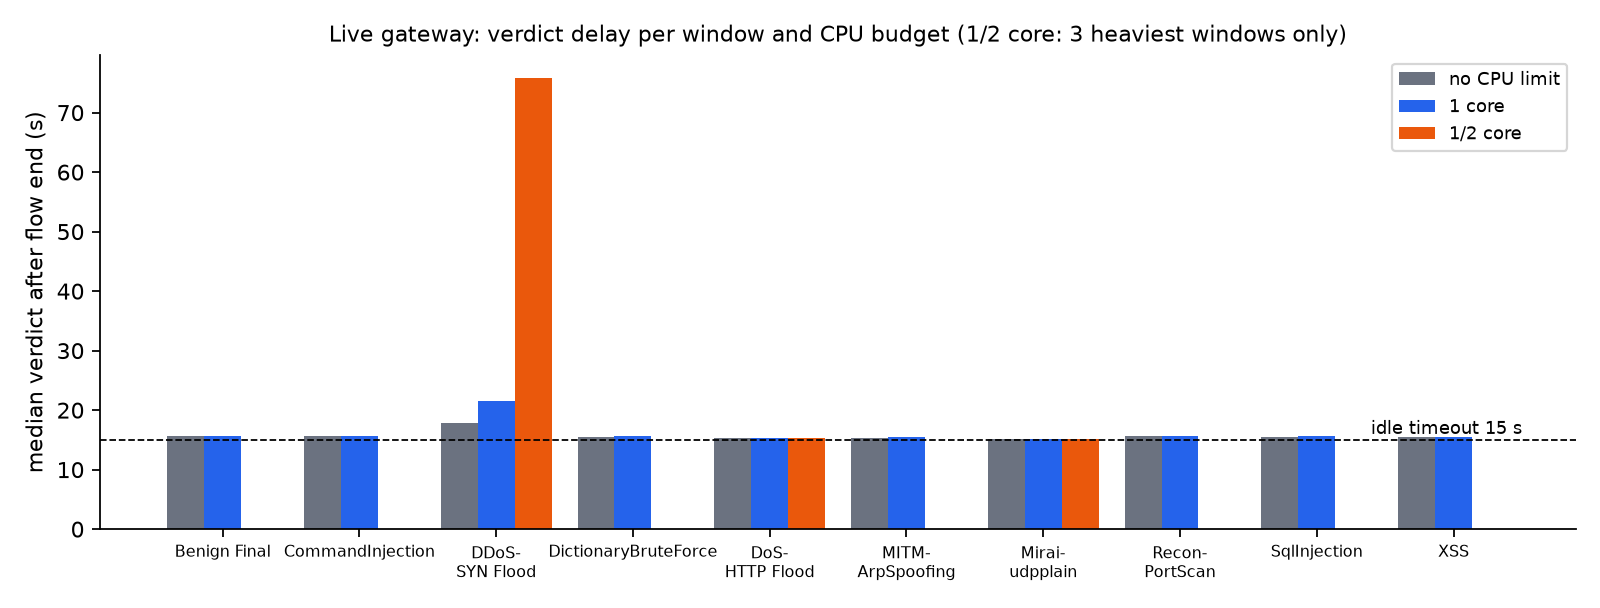
\includegraphics[width=\columnwidth]{../docs/figures/live_delay.png}
\caption{Median verdict delay after a flow's last packet, per window and CPU budget (legend ``1/2 core'': half a core, tested on the three heaviest windows only). Dashed: the 15\,s idle timeout.}
\label{fig:delay}
\end{figure}

\subsection{Failure Modes the Check Exposed}\label{sec:defect}

The fidelity numbers above hold only after three problems were fixed. None changed an offline score, since at end of file every remaining flow is flushed.

\emph{A forwarding pitfall.} Replayed frames carry the source MACs of many capture devices. A MAC-learning switch maps all of them to h1's port and never forwards frames addressed to them, so part of the traffic silently never reaches the detector. Packet accounting reveals this; one OVS rule that forwards everything from h1 to gw fixes it.

\emph{Idle meters.} NFStream checks a meter's timeouts only when that meter receives a packet, so idle flows can wait in a meter that receives none. We use one meter and run a 200\,pps keep-alive ping between h1 and h2 on a management subnet that is never scored or blocked.

\emph{An export-ordering defect.} Unpatched NFStream~6.6.0 delivered verdicts tens of seconds after the idle timeout. \texttt{NFCache}, an LRU \texttt{OrderedDict}, moves a key to the most-recently-used end only in \texttt{\_\_setitem\_\_}, but \texttt{consume()} updates an existing flow in place, so the cache stays in creation order. \texttt{meter\_scan()} expires flows from the head and stops at the first non-idle flow. One long-lived active flow, such as the keep-alive ping, therefore blocks the idle expiry of every flow behind it until its 120\,s active timeout. A one-line fix, \texttt{cache.move\_to\_end(flow\_key)} in the update branch, restores LRU order without changing flow boundaries or features, so offline comparisons cannot see the defect. It cut the per-window median delay after flow end from 82.5\,s to 15.6\,s (SQLi window) and from 49.2\,s to 15.5\,s (XSS). In the unpatched XSS run only 118 of 224 flows (64.5\% of the packets) had been exported when the run stopped; on a continuously running gateway they would be exported late, not lost. Pekar and Jozsa map NFStream to CICFlowMeter features and leave the causes of value differences, among them ``the specific mechanisms employed for updating and terminating flows'', out of scope~\cite{pekar2024integrity}. To our knowledge the cause of this defect was previously undiagnosed. We reported it as nfstream\#262~\cite{nfstream262} and submitted the fix with a regression test as PR~\#263~\cite{nfstream263}.\footnote{The symptom was reported without a cause in nfstream \#120 (2022)~\cite{nfstream120}.}
